% Options for packages loaded elsewhere
\PassOptionsToPackage{unicode}{hyperref}
\PassOptionsToPackage{hyphens}{url}
\PassOptionsToPackage{dvipsnames,svgnames,x11names}{xcolor}
%
\documentclass[
  10pt,
  letterpaper,
  twocolumn]{article}

\usepackage{amsmath,amssymb}
\usepackage{iftex}
\ifPDFTeX
  \usepackage[T1]{fontenc}
  \usepackage[utf8]{inputenc}
  \usepackage{textcomp} % provide euro and other symbols
\else % if luatex or xetex
  \usepackage{unicode-math}
  \defaultfontfeatures{Scale=MatchLowercase}
  \defaultfontfeatures[\rmfamily]{Ligatures=TeX,Scale=1}
\fi
\usepackage{lmodern}
\ifPDFTeX\else  
    % xetex/luatex font selection
    \setmainfont[]{Times New Roman}
\fi
% Use upquote if available, for straight quotes in verbatim environments
\IfFileExists{upquote.sty}{\usepackage{upquote}}{}
\IfFileExists{microtype.sty}{% use microtype if available
  \usepackage[]{microtype}
  \UseMicrotypeSet[protrusion]{basicmath} % disable protrusion for tt fonts
}{}
\makeatletter
\@ifundefined{KOMAClassName}{% if non-KOMA class
  \IfFileExists{parskip.sty}{%
    \usepackage{parskip}
  }{% else
    \setlength{\parindent}{0pt}
    \setlength{\parskip}{6pt plus 2pt minus 1pt}}
}{% if KOMA class
  \KOMAoptions{parskip=half}}
\makeatother
\usepackage{xcolor}
\setlength{\emergencystretch}{3em} % prevent overfull lines
\setcounter{secnumdepth}{-\maxdimen} % remove section numbering
% Make \paragraph and \subparagraph free-standing
\makeatletter
\ifx\paragraph\undefined\else
  \let\oldparagraph\paragraph
  \renewcommand{\paragraph}{
    \@ifstar
      \xxxParagraphStar
      \xxxParagraphNoStar
  }
  \newcommand{\xxxParagraphStar}[1]{\oldparagraph*{#1}\mbox{}}
  \newcommand{\xxxParagraphNoStar}[1]{\oldparagraph{#1}\mbox{}}
\fi
\ifx\subparagraph\undefined\else
  \let\oldsubparagraph\subparagraph
  \renewcommand{\subparagraph}{
    \@ifstar
      \xxxSubParagraphStar
      \xxxSubParagraphNoStar
  }
  \newcommand{\xxxSubParagraphStar}[1]{\oldsubparagraph*{#1}\mbox{}}
  \newcommand{\xxxSubParagraphNoStar}[1]{\oldsubparagraph{#1}\mbox{}}
\fi
\makeatother


\providecommand{\tightlist}{%
  \setlength{\itemsep}{0pt}\setlength{\parskip}{0pt}}\usepackage{longtable,booktabs,array}
\usepackage{calc} % for calculating minipage widths
% Correct order of tables after \paragraph or \subparagraph
\usepackage{etoolbox}
\makeatletter
\patchcmd\longtable{\par}{\if@noskipsec\mbox{}\fi\par}{}{}
\makeatother
% Allow footnotes in longtable head/foot
\IfFileExists{footnotehyper.sty}{\usepackage{footnotehyper}}{\usepackage{footnote}}
\makesavenoteenv{longtable}
\usepackage{graphicx}
\makeatletter
\def\maxwidth{\ifdim\Gin@nat@width>\linewidth\linewidth\else\Gin@nat@width\fi}
\def\maxheight{\ifdim\Gin@nat@height>\textheight\textheight\else\Gin@nat@height\fi}
\makeatother
% Scale images if necessary, so that they will not overflow the page
% margins by default, and it is still possible to overwrite the defaults
% using explicit options in \includegraphics[width, height, ...]{}
\setkeys{Gin}{width=\maxwidth,height=\maxheight,keepaspectratio}
% Set default figure placement to htbp
\makeatletter
\def\fps@figure{htbp}
\makeatother
% definitions for citeproc citations
\NewDocumentCommand\citeproctext{}{}
\NewDocumentCommand\citeproc{mm}{%
  \begingroup\def\citeproctext{#2}\cite{#1}\endgroup}
\makeatletter
 % allow citations to break across lines
 \let\@cite@ofmt\@firstofone
 % avoid brackets around text for \cite:
 \def\@biblabel#1{}
 \def\@cite#1#2{{#1\if@tempswa , #2\fi}}
\makeatother
\newlength{\cslhangindent}
\setlength{\cslhangindent}{1.5em}
\newlength{\csllabelwidth}
\setlength{\csllabelwidth}{3em}
\newenvironment{CSLReferences}[2] % #1 hanging-indent, #2 entry-spacing
 {\begin{list}{}{%
  \setlength{\itemindent}{0pt}
  \setlength{\leftmargin}{0pt}
  \setlength{\parsep}{0pt}
  % turn on hanging indent if param 1 is 1
  \ifodd #1
   \setlength{\leftmargin}{\cslhangindent}
   \setlength{\itemindent}{-1\cslhangindent}
  \fi
  % set entry spacing
  \setlength{\itemsep}{#2\baselineskip}}}
 {\end{list}}
\usepackage{calc}
\newcommand{\CSLBlock}[1]{\hfill\break\parbox[t]{\linewidth}{\strut\ignorespaces#1\strut}}
\newcommand{\CSLLeftMargin}[1]{\parbox[t]{\csllabelwidth}{\strut#1\strut}}
\newcommand{\CSLRightInline}[1]{\parbox[t]{\linewidth - \csllabelwidth}{\strut#1\strut}}
\newcommand{\CSLIndent}[1]{\hspace{\cslhangindent}#1}

\usepackage{sdss2020} % Uses Times Roman font (either newtx or times package)
\usepackage{url}
\usepackage{hyperref}
\usepackage{latexsym}
\usepackage{amsmath, amsthm, amsfonts}
\usepackage{algorithm, algorithmic}
\usepackage[dvipsnames]{xcolor} % colors
\newcommand{\mt}[1]{{\textcolor{blue}{#1}}}
\newcommand{\svp}[1]{{\textcolor{RedOrange}{#1}}}
\makeatletter
\@ifpackageloaded{caption}{}{\usepackage{caption}}
\AtBeginDocument{%
\ifdefined\contentsname
  \renewcommand*\contentsname{Table of contents}
\else
  \newcommand\contentsname{Table of contents}
\fi
\ifdefined\listfigurename
  \renewcommand*\listfigurename{List of Figures}
\else
  \newcommand\listfigurename{List of Figures}
\fi
\ifdefined\listtablename
  \renewcommand*\listtablename{List of Tables}
\else
  \newcommand\listtablename{List of Tables}
\fi
\ifdefined\figurename
  \renewcommand*\figurename{Figure}
\else
  \newcommand\figurename{Figure}
\fi
\ifdefined\tablename
  \renewcommand*\tablename{Table}
\else
  \newcommand\tablename{Table}
\fi
}
\@ifpackageloaded{float}{}{\usepackage{float}}
\floatstyle{ruled}
\@ifundefined{c@chapter}{\newfloat{codelisting}{h}{lop}}{\newfloat{codelisting}{h}{lop}[chapter]}
\floatname{codelisting}{Listing}
\newcommand*\listoflistings{\listof{codelisting}{List of Listings}}
\makeatother
\makeatletter
\makeatother
\makeatletter
\@ifpackageloaded{caption}{}{\usepackage{caption}}
\@ifpackageloaded{subcaption}{}{\usepackage{subcaption}}
\makeatother

\ifLuaTeX
  \usepackage{selnolig}  % disable illegal ligatures
\fi
\usepackage{bookmark}

\IfFileExists{xurl.sty}{\usepackage{xurl}}{} % add URL line breaks if available
\urlstyle{same} % disable monospaced font for URLs
\hypersetup{
  pdftitle={100 years of Pies vs.~Bars},
  colorlinks=true,
  linkcolor={blue},
  filecolor={Maroon},
  citecolor={Blue},
  urlcolor={Blue},
  pdfcreator={LaTeX via pandoc}}


\title{100 years of Pies vs.~Bars}
\vspace{-1in}
\date{}

\begin{document}
\maketitle


William Playfair introduced the pie and bar charts in the early 1800s,
and by the turn of the next century, strong opinions about the
effectiveness of alternative displays of the same data had been
publicized in textbooks and manuals. For instance, Eells (1926) quotes
two contemporary resources which discuss pie charts as ``not a desirable
form of presentation'' (Brinton 1914) and more strongly, ``an insult to
a man's intelligence'' (Karsten 1923). Brinton (1914) even identifies
that the ``sector method'' is common, but if horizontal bar methods were
used more frequently, they would be preferred for both speed and
accuracy. Eells (1926) also quotes an excerpt from an introductory
statistics textbook (Secrist 1925), which argues that pie charts require
more cognitive effort to use accurately than a comparable stacked bar
chart, calling pie diagrams ``clumsy and defective''. These insights
mirror today's status quo: pie charts are stubbornly common, even though
many design guidelines recommend against their use and a variety of
empirical studies identify problems with circular data representations .
Wickham (2013) previously noted the prescience of design guidelines
prior to empirical studies validating their recommendations across
different types of visualizations.

\subsection{The Dawn of Empirical
Graphics}\label{the-dawn-of-empirical-graphics}

Interestingly, the question of pies and bars motivated some of the first
empirical evaluations of charts, published in the Journal of the
American Statistical Association: Eells (1926), von Huhn (1927), and
Croxton and Stryker (1927). Experimenters approached the problem
head-on, directly asking participants to estimate quantities from
charts, and evaluated participants on accuracy, and in some cases,
speed. While more sophisticated testing methodologies have been
developed over the past century (Vanderplas, Cook, and Hofmann 2020),
studies are still conducted today using direct estimation approaches
(VanderPlas, Ryan, and Hofmann 2019). Now as then, the phrasing of
direct estimation questions is of primary importance: a simple
mathematical transformation of the estimated quantity can have an
outsized effect on the results.

The initial studies of the question of pies and bars failed to identify
a clear ``best chart'' across all situations, or even to clearly
identify in which situations pie charts or bar charts should be
preferred. Eells (1926) found that pie charts were read as accurately as
bar charts and with comparable speed. The simplified nature of the
experiment attracted critiques from von Huhn (1927); attached to these
criticisms is a short study previously run by Croxton which examined
estimates of the ratio between smaller and larger sectors of
two-category pie and bar charts; these contributions will be addressed
separately even though they are often cited as a single paper, even
within the JASA records. von Huhn (1927)'s paper provides several
examples which highlight concerns with the Eells study, and argues that
while pie charts may be better in certain simple situations, bar charts
are much more extensible and facilitate more advanced comparisons, but
does not include any experimental studies. Croxton's early experimental
data (attached to von Huhn (1927)) had a larger number of participants
than Eells (1926), but only tested two-category charts with only two
proportions: .25 and .4. In addition, Croxton's study elicited estimates
from participants as \(A/B\) comparisons, where \(A + B = 1\), while
Eells elicited estimates for \(A\) and \(B\) separately. This multi-year
back-and-forth conversation is interesting in part because it pinpoints
an early example of experimental statistical graphics as a discipline of
interest to statisticians for both personal investigation and as an
audience for the results.

Subsequently, Croxton and Stryker (1927) published additional data
assessing accuracy of estimates from pie and bar charts, varying number
of categories and orientation/alignment of sections. Croxton and Stryker
(1927) found that pie charts matched or surpassed bar charts in most
situations, across different scale alignment and in charts with up to 5
categories (though at 5 categories, differences were not statistically
significant). The final paper in this early set of comparisons was
Croxton and Stein (1932), which examined a variety of representations of
proportional data, but outside the context of a statistical chart; the
experimental stimuli, while applicable to charts, show a focus on
general perception (though published in JASA).

Experimental graphics studies seem to have largely gone unreported (if
they were conducted) between 1932 and the 1980s, particularly in
statistical publications, though the issue of pies and bars occasionally
pops up during this period in other disciplines.

\subsection{Modern Experimental
Graphics}\label{modern-experimental-graphics}

Much later, Cleveland and McGill (1984), a statistician and a
psychologist by training, respectively, conducted experiments on simple
graphical elements. These experiments were presented as supporting a
hierarchy of graphical perception which evolved over the course of the
sequence of studies. This ranking indicates that aligned length
judgments are more accurate than judgments based on area or angle, with
the implication that bar charts are more accurately perceived than pie
charts. While the full hierarchy of feature comprehension is often
assumed to be experimentally derived, the experiments presented in the
series of Cleveland \& McGill papers only inform a few elements of this
hierarchy. As in the late 1920s, the combination of introspection based
reasoning and a sequence of simple experiments did not go uncontested.
Spence and Lewandowsky (1991) (both psychologists) used forced-choice
questions of the form ``which is bigger, A or B+C'' to investigate the
accuracy of pie and bar charts for making part-to-whole comparisons. The
later studies show more of an interdisciplinary conversation around data
displays, which have become a general tool not limited to statisticians.
As a result, the literature becomes fragmented; studies are conducted
across different disciplines, with different methods, elicitation
questions, protocols, and ultimately, different conclusions.

\begin{figure}

\centering{

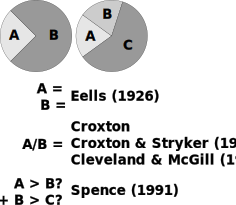
\includegraphics{pie-type-example.png}

}

\caption{\label{fig-elicitation}Different elicitation methods used to
assess accuracy of pie chart estimates.}

\end{figure}%

\subsection{Scope and Aims}\label{scope-and-aims}

In this study, we re-examine the historical literature surrounding the
use of pie and bar charts, including heuristics as well as empirical
studies. We trace guidelines back to experimental studies, where
possible, and examine whether justifications based on experimental
studies are in fact directly supported by those studies. We begin with
an initial set of four JASA papers from the late 1920s and early 1930s:
Eells (1926), Croxton and Stryker (1927), von Huhn (1927), and Croxton
and Stein (1932). We trace these studies forward in time, examining
papers which cite these studies, summaries of the original studies, and
any additional information provided relevant to pie and bar charts. In
addition, we specifically assess the different designs used in each
experimental study, examining how the type of elicitation method impacts
the results, as shown in Figure~\ref{fig-elicitation}. Synthesizing
these results, we use the fundamental question of ``which is better,
pies or bars?'' to examine the history of experimental graphics and
graphical design guidelines.{]}\{.svp\}

\section*{References}\label{references}
\addcontentsline{toc}{section}{References}

\phantomsection\label{refs}
\begin{CSLReferences}{1}{0}
\bibitem[\citeproctext]{ref-brintonGraphicMethodsPresenting1914}
Brinton, Willard Cope. 1914. \emph{Graphic Methods for Presenting
Facts}. New York, The Engineering Magazine Company.
\url{http://archive.org/details/graphicmethodsfo00brinrich}.

\bibitem[\citeproctext]{ref-clevelandGraphicalPerceptionTheory1984}
Cleveland, William S., and Robert McGill. 1984. {``Graphical Perception:
Theory, Experimentation, and Application to the Development of Graphical
Methods.''} \emph{Journal of the American Statistical Association} 79
(387): 531--54. \url{https://doi.org/10.1080/01621459.1984.10478080}.

\bibitem[\citeproctext]{ref-croxtonGraphicComparisonsBars1932}
Croxton, Frederick E., and Harold Stein. 1932. {``Graphic Comparisons by
Bars, Squares, Circles, and Cubes.''} \emph{Journal of the American
Statistical Association} 27 (177): 54--60.

\bibitem[\citeproctext]{ref-croxtonBarChartsCircle1927}
Croxton, Frederick E., and Roy E. Stryker. 1927. {``Bar Charts Versus
Circle Diagrams.''} \emph{Journal of the American Statistical
Association} 22 (160): 473--82. \url{https://doi.org/10.2307/2276829}.

\bibitem[\citeproctext]{ref-eellsRelativeMeritsCircles1926}
Eells, Walter Crosby. 1926. {``The Relative Merits of Circles and Bars
for Representing Component Parts.''} \emph{Journal of the American
Statistical Association} 21 (154): 119--32.
\url{https://doi.org/10.2307/2277140}.

\bibitem[\citeproctext]{ref-karsten1923charts}
Karsten, K. G. 1923. \emph{Charts and {Graphs}: {An Introduction} to
{Graphic Methods} in the {Control} and {Analysis} of {Statistics}}.
Prentice-Hall, Incorporated.
\url{https://books.google.com/books?id=DNc1AAAAIAAJ}.

\bibitem[\citeproctext]{ref-secristIntroductionStatisticalMethods1925}
Secrist, Horace. 1925. \emph{An {Introduction} to {Statistical Methods}:
{A Textbook} for {College Students}, a {Manual} for {Statisticians} and
{Business Executives}}. Macmillan.
\url{https://www.google.com/books/edition/An_Introduction_to_Statistical_Methods/cuUBAAAAMAAJ?hl=en}.

\bibitem[\citeproctext]{ref-spenceDisplayingProportionsPercentages1991}
Spence, I., and S. Lewandowsky. 1991. {``Displaying Proportions and
Percentages.''} \emph{Applied Cognitive Psychology} 5 (1): 61--77.
\url{https://doi.org/10.1002/acp.2350050106}.

\bibitem[\citeproctext]{ref-vanderplasTestingStatisticalCharts2020}
Vanderplas, Susan, Dianne Cook, and Heike Hofmann. 2020. {``Testing
{Statistical Charts}: {What Makes} a {Good Graph}?''} \emph{Annual
Review of Statistics and Its Application} 7 (1): 61--88.
\url{https://doi.org/10.1146/annurev-statistics-031219-041252}.

\bibitem[\citeproctext]{ref-vanderplasFramedReproducingRevisiting2019}
VanderPlas, Susan, Goluch C Ryan, and Heike Hofmann. 2019. {``Framed!
{Reproducing} and {Revisiting} 150-{Year-Old Charts}.''} \emph{Journal
of Computational and Graphical Statistics} 28 (3): 620--34.
\url{https://doi.org/10.1080/10618600.2018.1562937}.

\bibitem[\citeproctext]{ref-vonhuhnFurtherStudiesGraphic1927}
von Huhn, R. 1927. {``Further Studies in the Graphic Use of Circles and
Bars: A Discussion of the Eell's Experiment.''} \emph{Journal of the
American Statistical Association} 22 (157): 31--39.
\url{https://doi.org/10.2307/2277346}.

\bibitem[\citeproctext]{ref-wickhamGraphicalCriticismHistorical2013}
Wickham, Hadley. 2013. {``Graphical {Criticism}: {Some Historical
Notes}.''} \emph{Journal of Computational and Graphical Statistics} 22
(1): 38--44. \url{https://doi.org/10.1080/10618600.2012.761140}.

\end{CSLReferences}


\bibliographystyle{sdss2020} % Please do not change the bibliography style


\end{document}
